%%%%%%%%%%%%%%%%%%%%%%%%%%%%%%%%%%%%%%%%%%%%%%%%%%%%%%%%%%%
% Capitolo 3

\chapter{Ecosistemi mobili}
\label{ecosistemi}
I sistemi operativi per dispositivi mobili sono componenti software che garantiscono il funzionamento di dispositivi quali telefoni cellulari, smartphone, tablet, palmari e lettori MP3, coordinando e gestendo le risorse (hardware e software), e creando un'interfaccia con l'utente.
Diversamente dai sistemi operativi per desktop e laptop, essi devono affrontare problematiche critiche tra cui: limitatezza delle risorse (sia in termini di CPU che di memoria RAM), dimensioni ridotte dello schermo, sistemi touch-screen più o meno avanzati, tecnologie differenti per l'accesso ad Internet, consumo della batteria.
Nell'accezione moderna, il sistema operativo mobile non è solo un prodotto software, ma una vera e propria piattaforma, che mette a disposizione degli sviluppatori delle API su cui sviluppare applicazioni.

Un \emph{ecosistema mobile} è costituito dal sistema operativo, inteso come piattaforma, dagli sviluppatori, che incrementano il numero e migliorano la qualità delle applicazioni disponibili, e dagli utilizzatori, che acquistano sia la piattaforma che le applicazioni nello store.
In questo capitolo verranno trattate i principali sistemi operativi mobile e i relativi frameworks per lo sviluppo delle applicazioni.

\section{Sistemi operativi per dispositivi mobili}

Di seguito una breve descrizione dei sistemi operativi mobili più diffusi.

\subsection{Android}
Android (\emph{\url{http://www.android.com/}}), nato nel 2003, è il più diffuso sistema operativo per dispositivi mobili; open source; distribuito sotto licenza Apache, ovvero vi è la possibilità di modificare e distribuire liberamente il codice sorgente.\\
\begin{figure}
\begin{center}
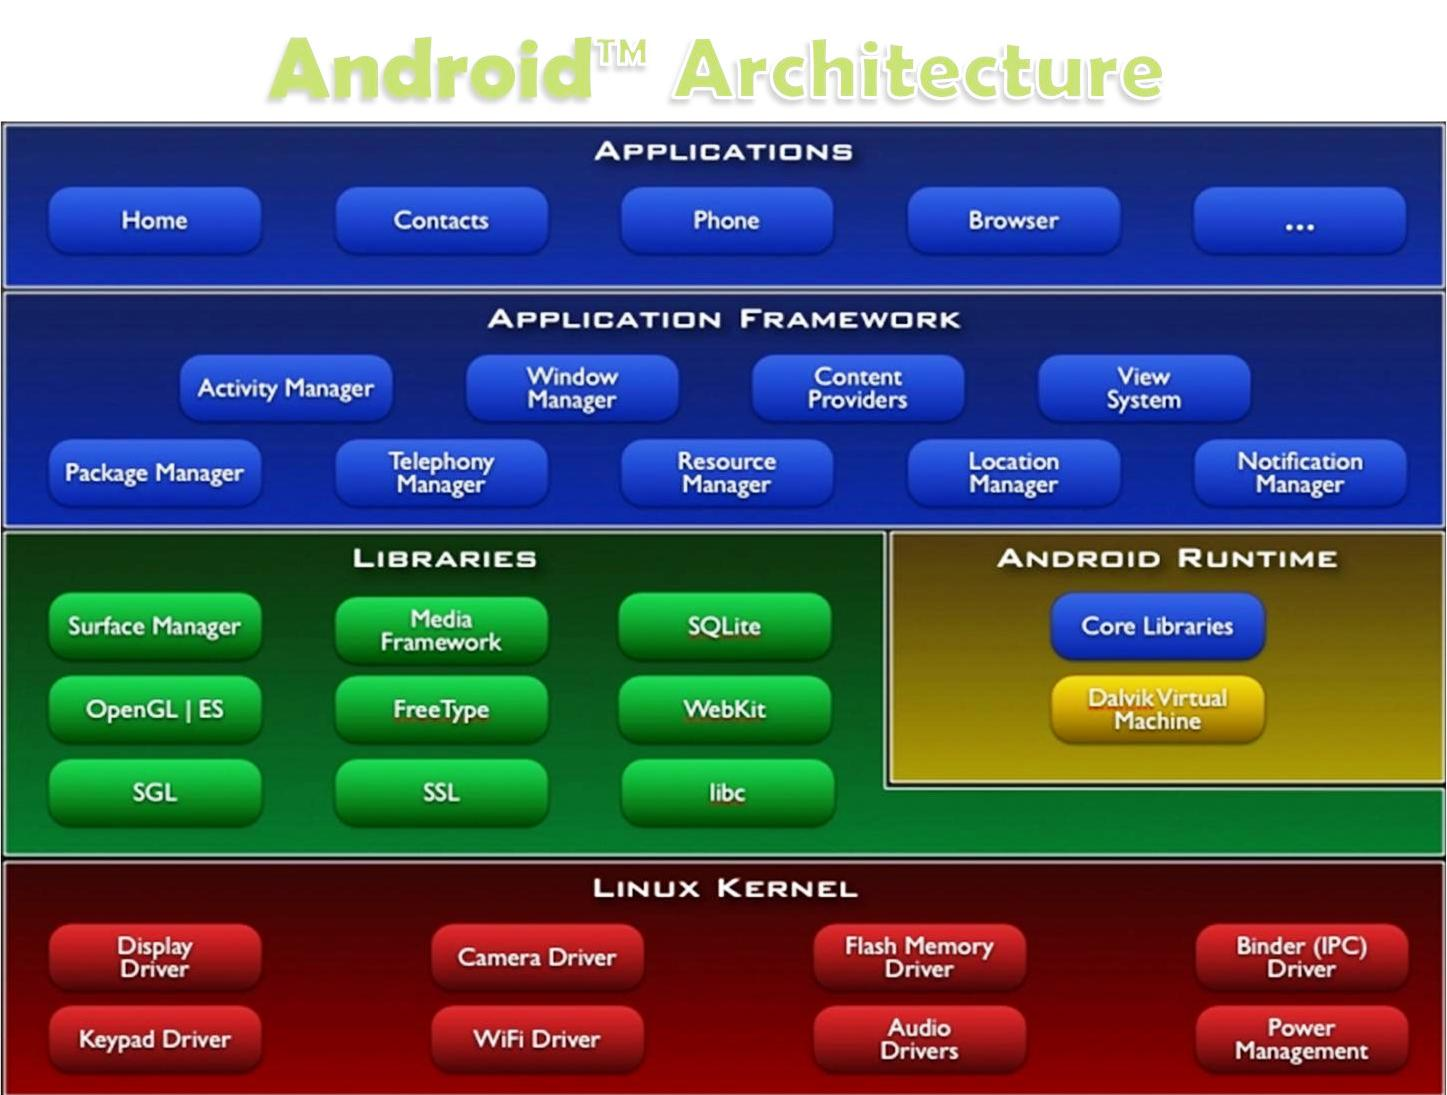
\includegraphics[scale=0.5]{imgs/android_architecture.jpg} 
\caption{Architettura del sistema operativo Android\label{androidarchitecture}}
\end{center}
\end{figure}

L'architettura Android, riportata in figura \ref{androidarchitecture}, è così definita:
\begin{itemize}
\item \emph{kernel}, basato sul kernel Linux(versioni 2.6 e 3.x), contiene i driver per il funzionamento del dispositivo;
\item \emph{strato middleware contenente Librerie ed API}: scritte in C o C++, sono le librerie che forniscono le funzionalità standard al dispositivo, ovvero gestione delle funzioni del display (Surface Manager), gestione dei media (Media Framework), fonts di sistema, DBMS (SQLite), web browser engine (WebKit), e numerose altre;
\item \emph{Android Runtime}: Contiene la Dalvik virtual machine, una macchina virtuale ottimizzata per sfruttare la poca memoria presente nei dispositivi mobili, e che consente di far girare diverse istanze della macchina virtuale contemporaneamente, nascondendo al sistema operativo sottostante la gestione della memoria e dei thread. E' presente, inoltre, un compilatore just-in-time che esegue il Dalvik dex-code, simile al bytecode Java;
\item \emph{Framework di applicazioni che include librerie java basate su Apache Harmony\footnote{Sito internet di riferimento http://harmony.apache.org/}},  costituito da una serie di componenti e API che eseguono numerosi compiti, tra i quali la gestione dell'interazione con l'utente (tramite l'Activity Manager), la condivisione delle informazioni tra i vari processi (Content Provider), gestione delle finestre (Window Manager), gestione delle funzionalità telefoniche (Telephony Manager), ottimizzazione delle risorse (Resource Manager), gestione del ciclo di vita delle applicazioni (Package Manager), gestione della localizzazione (Location Manager), gestione delle notifiche con l'utente (Notification Manager).
\end{itemize}

Per quanto riguarda gli aggiornamenti, Android ha un rapido ciclo di rilascio (nuove versioni ogni sei-nove mesi).
Gli aggiornamenti sono in genere di natura incrementale e apportano miglioramenti del software a intervalli regolari. Tra una major release e l'altra vengono messi a disposizione rilasci intermedi per risolvere problemi di sicurezza e altri bug del software.
\\


\subsubsection{Sviluppo Applicazioni}
Tutte le applicazioni Android, dovendo basarsi sul framework di librerie Java, sono scritte in Java.

L'Android software development kit SDK (\emph{\url{http://developer.android.com/sdk/}}) include un insieme di tool di sviluppo, quali un debugger, librerie, un emulatore basato su QEMU (\emph{\url{http://wiki.qemu.org/}}), codici di esempio e tutorials.
Le piattaforme di sviluppo supportate includono computer con sistema operativo Linux, MAC OS X (dalla 10.5.8) e Windows (da XP).
L'IDE (Integrated Development Enviroment) ufficialmente supportato è ADT (Android Development Tools), basato su Eclipse (\emph{\url{http://www.eclipse.org/}}) ma, in ogni caso, è possibile sviluppare applicazioni Android anche con altri IDE.

\subsection{iOS}
iOS (\emph{\url{http://www.apple.com/it/ios/}}) è un sistema operativo di Apple, derivato da Unix BSD ed ha un microkernel XNU Mach basato su Darwin OS.
Nato nel 2007, è rilasciato sotto licenza APSL (Apple Public Source License), che consente agli utenti di migliorare il software ma non di rilasciarlo.\\

\begin{figure}[h!]
\begin{center}
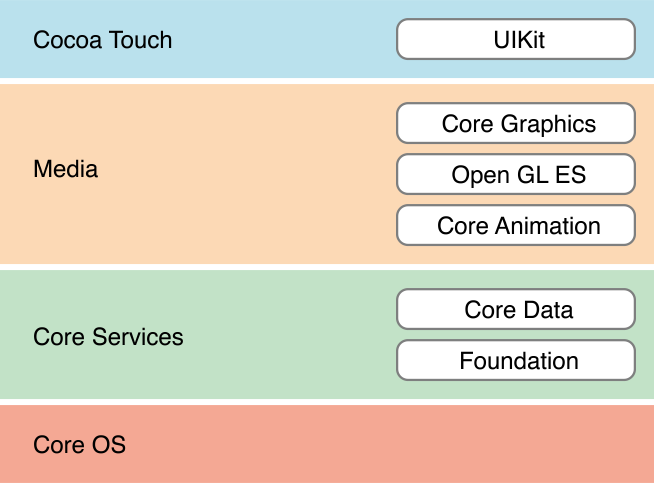
\includegraphics[scale=0.5]{imgs/ios_architecture.png} 
\caption{Architettura del sistema operativo iOS\label{iosarchitecture}}
\end{center}
\end{figure}

iOS ha quattro livelli di astrazione, riportati in figura \ref{iosarchitecture}:
\begin{itemize}
\item \emph{Core OS Layer}: contiene le caratteristiche di basso livello su cui sono basate la maggior parte delle tecnologie. Contiene il kernel ed interfacce di basso livello UNIX. Gestisce la memoria virtuale, i threads, il filesystem e i driver delle periferiche.
Sono presenti, inoltre, framework per l'esecuzione di DSP, calcoli di algebra lineare ed elaborazione delle immagini ; framework per la gestione del Bluetooth; framework per la gestione degli accessori hardware eventualmente connessi al dispositivo; framework per la sicurezza;
\item \emph{Core Services Layer}: contiene i servizi di sistema fondamentali che tutte le applicazioni usano. Offre quindi servizi di alto livello basati sui Core Service Frameworks, ad esempio lo storage di dati in remoto (iCloud); la protezione dei dati sensibili, per evitare che applicazioni malevole facciano uso di essi; la gestione dei documenti XML; la possibilità di condividere dati tra le varie applicazioni;
\item \emph{Media Layer}: contiene le tecnologie grafiche, audio e video;
\item \emph{Cocoa Touch Layer}: contiene i framework indispensabili per costruire applicazioni iOS (Cocoa Service Framework) e definisce l'infrastruttura di base ed il supporto per tecnologie fondamentali come il multitasking, l'input basato sul touch, le notifiche in push e locali e molti altri servizi di alto livello.
\end{itemize}

Apple rilascia aggiornamenti di iOS circa una volta l'anno. Tali aggiornamenti costituiscono revisioni complete del sistema operativo.
\subsubsection{Sviluppo Applicazioni}
Le applicazioni per iOS possono essere sviluppate tramite l'iOS SDK (\emph{\url{http://developer.apple.com/}}),  disponibile solo su sistema operativo MAC OS X. Esse sono scritte in Objective-C, anche se esiste il supporto per C e C++.

L'IDE di riferimento per lo sviluppo di applicazioni per iOS è XCode, che include un editor di sorgenti; uno strumento per disegnare le interfacce utente; il compilatore LLVM  e un emulatore, oltre ad altri numerosi tool per il debug, il testing e la gestione degli errori.


\subsection{Windows Phone OS}
Windows Phone OS (\emph{\url{http://www.windowsphone.com/it-it}}) è un sistema operativo Microsoft, nato nel 2010, orientato ai dispositivi mobile. E' il successore di Windows Mobile, sistema operativo nato nel 1996 per i palmari, ma è completamente differente da quest'ultimo.

E' distribuito con licenza Microsoft EULA, per cui è soggetto a limitazioni d'uso, di garanzia e di responsabilità.

\begin{figure}
\begin{center}
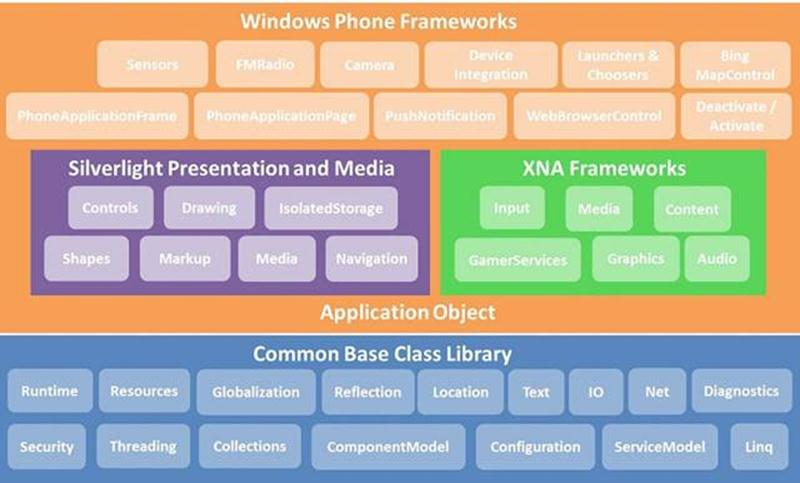
\includegraphics[scale=0.7]{imgs/windowsphone_architecture.jpg} 
\caption{Architettura del sistema operativo iOS\label{wparchitecture}}
\end{center}
\end{figure}

Windows Phone OS ha un'architettura a quattro livelli, come rappresentato in figura \ref{wparchitecture}:
\begin{itemize}
\item \emph{Common Base Class Library}: è una libreria standard che include un vasto numero di funzionalità comuni, come ad esempio la lettura e scrittura su un file, il rendering grafico, l'interazione con i database, la manipolazione di documenti XML e il supporto per il multithreading;
\item \emph{Silverlight Presentation and Media}: fornisce librerie per la navigazione, la grafica, la gestione dei media;
\item \emph{XNA Frameworks}: è un insieme di librerie, servizi e risorse per la gestione dell'accelerazione grafica e del rendering, dell'audio e dei servizi di autenticazione e connettività;
\item \emph{Windows Phone Frameworks}: definisce dei blocchi comuni per tutte le applicazioni Windows Phone. Esso fornisce l'interfaccia al sistema ed alle risorse hardware, ovvero i sensori, l'accelerometro, il compasso, il giroscopio e la fotocamera. In Windows Phone Framework è presente anche un sistema di notifiche.
\end{itemize}

\subsubsection{Sviluppo Applicazioni}
Le applicazioni per Windows Phone possono essere scritte in C++, C\#, C, Visual Basic e HTML5, grazie al vasto supporto del framework .NET.
La più recente versione della Windows Phone SDK (\emph{\url{http://dev.windowsphone.com/}}) è disponibile solo per sistemi operativi Windows 8 a 64bit.

L'IDE di riferimento per lo sviluppo di applicazioni Windows Phone è Visual Studio per Windows Phone, che include un editor di sorgenti, di testing, di debug, di gestione delle risorse e del ciclo di vita dell'applicazione.
Microsoft mette inoltre a disposizione altri significativi tools come Express Blend, che permette di creare interfacce utente; Silverlight (\emph{\url{http://www.microsoft.com/silverlight/}}) e XNA per la gestione della grafica 2D e 3D; Windows Phone Emulator, l'emulatore dei dispositivi Windows Phone.\\


\clearpage{\pagestyle{empty}\cleardoublepage}